\documentclass{standalone}
\usepackage{graphicx}
\usepackage{pgfplots}
\usepackage{tikz}

\usepackage{amsmath,amsfonts,amssymb}
\usetikzlibrary{calc}
%\pgfplotsset{compat=1.7, cell picture=if necessary}

% Las imagenes de esta carpeta se obtienen cambiado el parametro

\usetikzlibrary{arrows,decorations.markings}

%\usetikzlibrary{quotes,angles}

\usetikzlibrary{patterns}
\usetikzlibrary{decorations.pathreplacing}

\begin{document}
	
\tiny

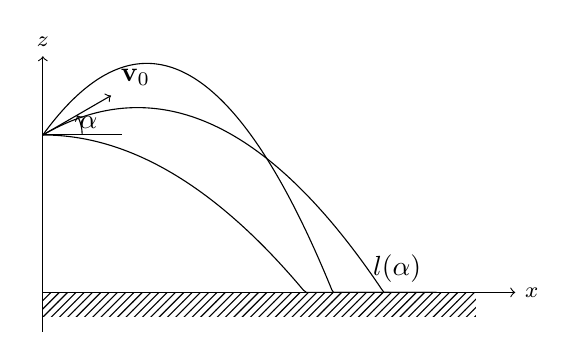
\begin{tikzpicture}
	\def\pinum{3.14159}
	\def\phi{3*\pi/4}
	\def\R{1}
	

	\draw[->] (0,0)--(6,0) node [right] {\footnotesize $x$};
	
	\draw[->] (0,-.5)-- (0,3) node [above]{\footnotesize $z$} ;

	\pattern[pattern = north east lines] (0,0) rectangle (5.5, -0.3) ;
	
	\def \h {2}
	\def \g {9}
	\def \vzero {5}
	
	\def \alphanum {0.9*\pinum/3}
	\draw[variable=\t,domain=0:1.5,samples=200]
	plot (		{\vzero*cos(\alphanum r)*\t},			{max(\h + \vzero*sin(\alphanum r)*\t - \g*\t *\t / 2 ,0 )}	)
	;
	
	\def \alphanum {\pinum/6}
	\draw[variable=\t,domain=0:1.5,samples=200]
	plot (		{min(\vzero*cos(\alphanum r)*\t , 5)},			{max(\h + \vzero*sin(\alphanum r)*\t - \g*\t *\t / 2 ,0 )}	)
	;
	
	\draw[->] (0,\h) -- ($({cos(\alphanum r)},{\h + sin(\alphanum r)})$) node [above right] {$\mathbf v _0$};

	\draw (0,\h) -- (1,\h);
	
	\def \rnum {.5}

	\draw[->] (0,\h) + (\rnum,0)  arc ({0}:{\alphanum*180/\pinum}:\rnum cm) ;
	\node[] at ($(0,\h)+ ({.5*\alphanum*180/\pinum}:{\rnum + .1})$) {$\alpha$};
	
	\node [above] at (4.5,0) {$l(\alpha)$};

	\def \alphanum {0}
	\draw[variable=\t,domain=0:1.5,samples=200]
	plot (		{min(\vzero*cos(\alphanum r)*\t , 5)},			{max(\h + \vzero*sin(\alphanum r)*\t - \g*\t *\t / 2 ,0 )}	)
	;
	

	
	
	
\end{tikzpicture} 


\end{document}